
\documentclass[sigconf]{acmart}
\usepackage{lipsum}
%%
%% \BibTeX command to typeset BibTeX logo in the docs
\AtBeginDocument{%
  \providecommand\BibTeX{{%
    Bib\TeX}}}

%% Rights management information.  This information is sent to you
%% when you complete the rights form.  These commands have SAMPLE
%% values in them; it is your responsibility as an author to replace
%% the commands and values with those provided to you when you
%% complete the rights form.
\setcopyright{acmlicensed}
\copyrightyear{2024}
\acmYear{2024}
\acmDOI{XXXXXXX.XXXXXXX}

%% These commands are for a PROCEEDINGS abstract or paper.
\acmConference[iWOAR]{international Workshop on Sensor-Based Activity Recognition and Artificial Intelligence}{September 26--27,
  2024}{Potsdam, DE}
%%
%%  Uncomment \acmBooktitle if the title of the proceedings is different
%%  from ``Proceedings of ...''!
%%
%%\acmBooktitle{Woodstock '18: ACM Symposium on Neural Gaze Detection,
%%  June 03--05, 2018, Woodstock, NY}
\acmISBN{978-1-4503-XXXX-X/18/06}


%%
%% Submission ID.
%% Use this when submitting an article to a sponsored event. You'll
%% receive a unique submission ID from the organizers
%% of the event, and this ID should be used as the parameter to this command.
%%\acmSubmissionID{123-A56-BU3}

%%
%% For managing citations, it is recommended to use bibliography
%% files in BibTeX format.
%%
%% You can then either use BibTeX with the ACM-Reference-Format style,
%% or BibLaTeX with the acmnumeric or acmauthoryear sytles, that include
%% support for advanced citation of software artefact from the
%% biblatex-software package, also separately available on CTAN.
%%
%% Look at the sample-*-biblatex.tex files for templates showcasing
%% the biblatex styles.
%%

%%
%% The majority of ACM publications use numbered citations and
%% references.  The command \citestyle{authoryear} switches to the
%% "author year" style.
%%
%% If you are preparing content for an event
%% sponsored by ACM SIGGRAPH, you must use the "author year" style of
%% citations and references.
%% Uncommenting
%% the next command will enable that style.
%%\citestyle{acmauthoryear}


%%
%% end of the preamble, start of the body of the document source.
\begin{document}

\title{Stairs vs Lift detector}


\author{Hrishikesh}
\email{hrishikesk.raoshaeb.com}
\affiliation{%
  \institution{Universität Siegen}
  \city{Siegen}
  \state{NRW}
  \country{Germany}
}

\author{Ravi}
\email{ravikiran.arasur.com}
\affiliation{%
  \institution{Universität Siegen}
  \city{Siegen}
  \state{NRW}
  \country{Germany}
}

\author{Nassim}
\email{nassim.com}
\affiliation{%
  \institution{Universität Siegen}
  \city{Siegen}
  \state{NRW}
  \country{Germany}
}

\author{Iman}
\email{iman.com}
\affiliation{%
  \institution{Universität Siegen}
  \city{Siegen}
  \state{NRW}
  \country{Germany}
}

\author{Nirav}
\email{nirav.com}
\affiliation{%
  \institution{Universität Siegen}
  \city{Siegen}
  \state{NRW}
  \country{Germany}
}

\author{Kristof van laherhoven}
\email{kvl.com}
\affiliation{%
  \institution{Universität Siegen}
  \city{Siegen}
  \state{NRW}
  \country{Germany}
}


%%
%% The abstract is a short summary of the work to be presented in the
%% article.
\begin{abstract}
\lipsum[1]
\end{abstract}

%%
%% The code below is generated by the tool at http://dl.acm.org/ccs.cfm.
%% Please copy and paste the code instead of the example below.
%%
\begin{CCSXML}
<ccs2012>
 <concept>
  <concept_id>00000000.0000000.0000000</concept_id>
  <concept_desc>Do Not Use This Code, Generate the Correct Terms for Your Paper</concept_desc>
  <concept_significance>500</concept_significance>
 </concept>
 <concept>
  <concept_id>00000000.00000000.00000000</concept_id>
  <concept_desc>Do Not Use This Code, Generate the Correct Terms for Your Paper</concept_desc>
  <concept_significance>300</concept_significance>
 </concept>
 <concept>
  <concept_id>00000000.00000000.00000000</concept_id>
  <concept_desc>Do Not Use This Code, Generate the Correct Terms for Your Paper</concept_desc>
  <concept_significance>100</concept_significance>
 </concept>
 <concept>
  <concept_id>00000000.00000000.00000000</concept_id>
  <concept_desc>Do Not Use This Code, Generate the Correct Terms for Your Paper</concept_desc>
  <concept_significance>100</concept_significance>
 </concept>
</ccs2012>
\end{CCSXML}

\ccsdesc[500]{Do Not Use This Code~Generate the Correct Terms for Your Paper}
\ccsdesc[300]{Do Not Use This Code~Generate the Correct Terms for Your Paper}
\ccsdesc{Do Not Use This Code~Generate the Correct Terms for Your Paper}
\ccsdesc[100]{Do Not Use This Code~Generate the Correct Terms for Your Paper}

%%
%% Keywords. The author(s) should pick words that accurately describe
%% the work being presented. Separate the keywords with commas.
\keywords{Multiple, Keywords}

%%
%% This command processes the author and affiliation and title
%% information and builds the first part of the formatted document.
\maketitle

\section{Introduction}
the ``\verb|acmart|'' document class can
be used to prepare many different kinds of documentation --- a
double-anonymous initial submission of a full-length technical paper, a
two-page SIGGRAPH Emerging Technologies abstract, a ``camera-ready''
journal article, a SIGCHI Extended Abstract, and more --- all by
selecting the appropriate {\itshape template style} and {\itshape
  template parameters}. \url{https://www.acm.org/publications/proceedings-template}.

\section{Methodology}
\lipsum[4-5]
\subsection{Styles}
{\verb|acmsmall|} template style:
\begin{itemize}
\item {\texttt{acmsmall}}: The default journal template style.
\item {\texttt{acmlarge}}: Used by JOCCH and TAP.
\item {\texttt{acmtog}}: Used by TOG.
\end{itemize}

The majority of conference proceedings documentation will use the {\verb|acmconf|} template style.
\begin{itemize}
\item {\texttt{sigconf}}: The default proceedings template style.
\item{\texttt{sigchi}}: Used for SIGCHI conference articles.
\item{\texttt{sigplan}}: Used for SIGPLAN conference articles.
\end{itemize}

\subsection{Template Parameters}

Frequently-used parameters, or combinations of parameters, include:
\begin{itemize}
\item {\texttt{anonymous,review}}: Suitable for a ``double-anonymous''
  conference submission. Anonymizes the work and includes line
  numbers. Use with the \texttt{\acmSubmissionID} command to print the
  submission's unique ID on each page of the work.
\item{\texttt{authorversion}}: Produces a version of the work suitable
  for posting by the author.
\item{\texttt{screen}}: Produces colored hyperlinks.
\end{itemize}

\section{Results}
\lipsum[6-7]

Modifying the template --- including but not limited to: adjusting
margins, typeface sizes, line spacing, paragraph and list definitions,
and the use of the \verb|\vspace| --- is not allowed.
{\bfseries Your document will be returned to you for revision if
  modifications are discovered.}
\subsection{Subsection}
\lipsum[8]

 Use the {\verb|title|} command to define the title of
your work. If your work has a subtitle, define it with the
{\verb|subtitle|} command.  Do not insert line breaks in your title.

If your title is lengthy, you must define a short version to be used
in the page headers, to prevent overlapping text. The \verb|title|
command has a ``short title'' parameter:
\begin{verbatim}
  \title[short title]{full title}
\end{verbatim}

\section{Discussion}
\lipsum[9-10]

\section{Conclusion}
\lipsum[11]

\section{Authors and Affiliations}

The \verb|authornote| and \verb|authornotemark| commands allow a note
to apply to multiple authors --- for example, if the first two authors
of an article contributed equally to the work.

If your author list is lengthy, you must define a shortened version of
the list of authors. The following command should be placed just after
the last \verb|\author{}| definition:
\begin{verbatim}
  \renewcommand{\shortauthors}{McCartney, et al.}
\end{verbatim}

Note that authors' addresses are mandatory for journal articles.

\section{Tables}

The ``\verb|acmart|'' document class includes the ``\verb|booktabs|''
package --- \url{https://ctan.org/pkg/booktabs} --- for preparing
high-quality tables.

Table captions are placed {\itshape above} the table.

Because tables cannot be split across pages, the best placement for
them is typically the top of the page nearest their initial cite.  To
ensure this proper ``floating'' placement of tables, use the
environment \textbf{table} to enclose the table's contents and the
table caption.  The contents of the table itself must go in the
\textbf{tabular} environment, to be aligned properly in rows and
columns, with the desired horizontal and vertical rules.  Again,
detailed instructions on \textbf{tabular} material are found in the
\textit{\LaTeX\ User's Guide}.

Immediately following this sentence is the point at which
Table~\ref{tab:freq} is included in the input file; compare the
placement of the table here with the table in the printed output of
this document.

\begin{table}
  \caption{Frequency of Special Characters}
  \label{tab:freq}
  \begin{tabular}{ccl}
    \toprule
    Non-English or Math&Frequency&Comments\\
    \midrule
    \O & 1 in 1,000& For Swedish names\\
    $\pi$ & 1 in 5& Common in math\\
    \$ & 4 in 5 & Used in business\\
    $\Psi^2_1$ & 1 in 40,000& Unexplained usage\\
  \bottomrule
\end{tabular}
\end{table}

To set a wider table, which takes up the whole width of the page's
live area, use the environment \textbf{table*} to enclose the table's
contents and the table caption.  As with a single-column table, this
wide table will ``float'' to a location deemed more
desirable. Immediately following this sentence is the point at which
Table~\ref{tab:commands} is included in the input file; again, it is
instructive to compare the placement of the table here with the table
in the printed output of this document.

\begin{table*}
  \caption{Some Typical Commands}
  \label{tab:commands}
  \begin{tabular}{ccl}
    \toprule
    Command &A Number & Comments\\
    \midrule
    \texttt{{\char'134}author} & 100& Author \\
    \texttt{{\char'134}table}& 300 & For tables\\
    \texttt{{\char'134}table*}& 400& For wider tables\\
    \bottomrule
  \end{tabular}
\end{table*}

Always use midrule to separate table header rows from data rows, and
use it only for this purpose. This enables assistive technologies to
recognise table headers and support their users in navigating tables
more easily.

\section{Math Equations}
You may want to display math equations in three distinct styles:
inline, numbered or non-numbered display.  Each of the three are
discussed in the next sections.

\subsection{Inline (In-text) Equations}
A formula that appears in the running text is called an inline or
in-text formula.  It is produced by the \textbf{math} environment,
which can be invoked with the usual
\texttt{{\char'134}begin\,\ldots{\char'134}end} construction or with
the short form \texttt{\$\,\ldots\$}. You can use any of the symbols
and structures, from $\alpha$ to $\omega$, available in
\LaTeX~\cite{Lamport:LaTeX}; this section will simply show a few
examples of in-text equations in context. Notice how this equation:
\begin{math}
  \lim_{n\rightarrow \infty}x=0
\end{math},
set here in in-line math style, looks slightly different when
set in display style.  (See next section).

\subsection{Display Equations}
A numbered display equation---one set off by vertical space from the
text and centered horizontally---is produced by the \textbf{equation}
environment. An unnumbered display equation is produced by the
\textbf{displaymath} environment.

Again, in either environment, you can use any of the symbols and
structures available in \LaTeX\@; this section will just give a couple
of examples of display equations in context.  First, consider the
equation, shown as an inline equation above:
\begin{equation}
  \lim_{n\rightarrow \infty}x=0
\end{equation}
Notice how it is formatted somewhat differently in
the \textbf{displaymath}
environment.  Now, we'll enter an unnumbered equation:
\begin{displaymath}
  \sum_{i=0}^{\infty} x + 1
\end{displaymath}
and follow it with another numbered equation:
\begin{equation}
  \sum_{i=0}^{\infty}x_i=\int_{0}^{\pi+2} f
\end{equation}
just to demonstrate \LaTeX's able handling of numbering.


\section*{Acknowledgments}
\lipsum[12]









\section{Figures}

The ``\verb|figure|'' environment should be used for figures. One or
more images can be placed within a figure. If your figure contains
third-party material, you must clearly identify it as such, as shown
in the example below.
\begin{figure}[h]
  \centering
  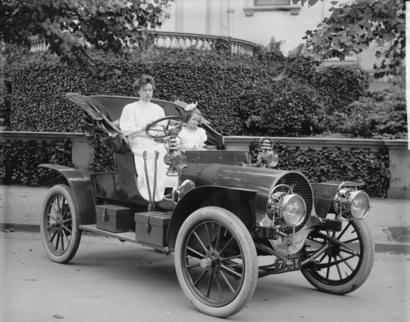
\includegraphics[width=\linewidth]{sample-franklin}
  \caption{1907 Franklin Model D roadster. Photograph by Harris \&
    Ewing, Inc. [Public domain], via Wikimedia
    Commons. (\url{https://goo.gl/VLCRBB}).}
  \Description{A woman and a girl in white dresses sit in an open car.}
\end{figure}

Your figures should contain a caption which describes the figure to
the reader.

Figure captions are placed {\itshape below} the figure.

Every figure should also have a figure description unless it is purely
decorative. These descriptions convey what’s in the image to someone
who cannot see it. They are also used by search engine crawlers for
indexing images, and when images cannot be loaded.


\section{Citations and Bibliographies}

The use of \BibTeX\ for the preparation and formatting of one's
references is strongly recommended. Authors' names should be complete
--- use full first names (``Donald E. Knuth'') not initials
(``D. E. Knuth'') --- and the salient identifying features of a
reference should be included: title, year, volume, number, pages,
article DOI, etc.

The bibliography is included in your source document with these two
commands, placed just before the \verb|\end{document}| command:
\begin{verbatim}
  \bibliographystyle{ACM-Reference-Format}
  \bibliography{bibfile}
\end{verbatim}
where ``\verb|bibfile|'' is the name, without the ``\verb|.bib|''
suffix, of the \BibTeX\ file.

Citations and references are numbered by default. A small number of
ACM publications have citations and references formatted in the
``author year'' style; for these exceptions, please include this
command in the {\bfseries preamble} (before the command
``\verb|\begin{document}|'') of your \LaTeX\ source:
\begin{verbatim}
  \citestyle{acmauthoryear}
\end{verbatim}


  Some examples.  A paginated journal article \cite{Abril07}, an
  enumerated journal article \cite{Cohen07}, a reference to an entire
  issue \cite{JCohen96}, a monograph (whole book) \cite{Kosiur01}, a
  monograph/whole book in a series (see 2a in spec. document)
  \cite{Harel79}, a divisible-book such as an anthology or compilation
  \cite{Editor00} followed by the same example, however we only output
  the series if the volume number is given \cite{Editor00a} (so
  Editor00a's series should NOT be present since it has no vol. no.),
  a chapter in a divisible book \cite{Spector90}, a chapter in a
  divisible book in a series \cite{Douglass98}, a multi-volume work as
  book \cite{Knuth97}, a couple of articles in a proceedings (of a
  conference, symposium, workshop for example) (paginated proceedings
  article) \cite{Andler79, Hagerup1993}, a proceedings article with
  all possible elements \cite{Smith10}, an example of an enumerated
  proceedings article \cite{VanGundy07}, an informally published work
  \cite{Harel78}, a couple of preprints \cite{Bornmann2019,
    AnzarootPBM14}, a doctoral dissertation \cite{Clarkson85}, a
  master's thesis: \cite{anisi03}, an online document / world wide web
  resource \cite{Thornburg01, Ablamowicz07, Poker06}, a video game
  (Case 1) \cite{Obama08} and (Case 2) \cite{Novak03} and \cite{Lee05}
  and (Case 3) a patent \cite{JoeScientist001}, work accepted for
  publication \cite{rous08}, 'YYYYb'-test for prolific author
  \cite{SaeediMEJ10} and \cite{SaeediJETC10}. Other cites might
  contain 'duplicate' DOI and URLs (some SIAM articles)
  \cite{Kirschmer:2010:AEI:1958016.1958018}. Boris / Barbara Beeton:
  multi-volume works as books \cite{MR781536} and \cite{MR781537}. A
  couple of citations with DOIs:
  \cite{2004:ITE:1009386.1010128,Kirschmer:2010:AEI:1958016.1958018}. Online
  citations: \cite{TUGInstmem, Thornburg01, CTANacmart}.
  Artifacts: \cite{R} and \cite{UMassCitations}.

\begin{acks}
Identification of funding sources and other support, and thanks to
individuals and groups that assisted in the research and the
preparation of the work should be included in an acknowledgment
section, which is placed just before the reference section in your
document.

This section has a special environment:
\begin{verbatim}
  \begin{acks}
  ...
  \end{acks}
\end{verbatim}
so that the information contained therein can be more easily collected
during the article metadata extraction phase, and to ensure
consistency in the spelling of the section heading.

Authors should not prepare this section as a numbered or unnumbered {\verb|\section|}; please use the ``{\verb|acks|}'' environment.
\end{acks}


\bibliographystyle{ACM-Reference-Format}
\bibliography{sample-base}


\end{document}

